\chapter{Security Aspects}
\label{chap:5}
%
Fully autonomous cars are not quite ready to go into the roads yet, but autonomous vehicles are getting closer to reality more than ever before. More than $60$ cities in the world have testing programs for autonomous cars or in preparation for it. Around $80$\$ billion is already invested in the technology, and almost every modern vehicle manufacturer has dedicated some resources for more and more automation in the newly launched car [??].  According to statistics [??] around $130k$ cars with partial automation are sold yearly and with current predictions until $2020$ around $98k$ fully automated vehicles will be sold. Until $2040$ this number is expected to be more than $96$ million, which represents $95$\% of all vehicles sold. \\
Without a big novelty in technology, autonomous cars are promising enhanced safety and improved convenience, however, it still has a darker side. Autonomous cars essentially can be called Internet cars and being high-tech vehicles they have vulnerabilities and a lot of security issues. This chapter aim is to get to the bottom of potential security risks and defense strategies.

\section{Background}

As autonomous vehicles are getting closer to reality as private and public transit vehicles, it is natural to be interested in safety and security which these new technologies are promising. One report made by FBI brought out a number of security vulnerabilities and concerns related to autonomous vehicles, stating that autonomous technologies can become a potentially deadly weapon in the future [??]. But greater concern than terrorism attacks on autonomous vehicles are the risk of controls systems being hacked in and taking control of a driving or other essential systems and in this way to put into a dangerous situation driver or passengers of the car. Overtaking a control of the car can be used to consciously cause an accident or to drive a car into all new unplanned location and potentially steal a car using technologies. It also can allow lock passengers inside against their will. Or to track the car user and make a profile of the person, who is driving/using a car. In fact, autonomous cars technology are still quite new and it is still hard to see the full scope for security risks of autonomous vehicles. \\
This can sound too non-realistic, but white hat hackers for years already have been showing security issues related to connected cars, demonstrating how easy is to take control and do harm over a lot of various systems even in non-automated vehicles. All these vulnerabilities connected to the Internet are open to various kind of attacks. Even advanced autopilot system, designed by Tesla can be tricked quite easily. One of Chinese security company demonstrated that it is very easy to spoof sensors of a vehicle, causing them to sense "ghost" objects or fail to detect a real object at all [??].
Here natural question can arise, so what makes autonomous vehicles so vulnerable against malicious attacks as compared with non- or only partial autonomous cars? Authors of \cite{sec} suggesting two main reasons:
\begin{enumerate}
	\item \textbf{The increased interaction between autonomous cars and environment.} At the moment the most communications between vehicles on the road occurs via \glspl{VANET}. This type of communication allows sharing fast changing surrounding information with vehicles which are nearby communicating vehicle. This allows for other cars/drivers in the cars to be aware of what is the road situation nearby them \cite{carspeak}. Since technologies are improving and fully autonomous cars will be on the roads in the very near future, \gls{V2I} and \gls{V2IoT} communication will be more common on the roads. Due to connectivity in one network, only one "infected" vehicle can compromise the entire network if the network is not properly secured.
	\item \textbf{The increased interaction between components of the system inside, so-called intra vehicular communication.} Autonomous cars have a lot of different \glspl{ECU} which are connected with each other using \gls{CAN} bus. One of the biggest advantages of using \gls{CAN} bus is that it is like a central unit into which a lot of different modules can be added or removed without changing the wiring architecture in the car. \gls{CAN} has three main parts:  \textbf{Data link layer}, which is responsible for data transferring. \textbf{High speed} physical layer and \textbf{Low speed} physical layer which is also responsible for fault toleration. In most cases, the most important control units (which has a direct impact on safety, e.g. brake or engine control module) are connected to high speed layer and others, not so security sensitive are connected to low speed layer. Not so common situation, but it is possible to have a "gateway bridge" which opens the route for selected packages from low to high (or vice versa) layers. So it is a possibility that that malicious packets are connected to the \gls{CAN} bus using low speed layer and without any further checking or suspicion it can be transferred into high speed layer causing to serious consequences. Control architecture in autonomous vehicles is working in this way what all nodes get packages from \gls{CAN}. Any malicious component which is connected to the internal vehicle network can snoop all communications or it can infect all other elements. In order to protect the network, every path for package moving should be protected to ensure the vehicle security. Unfortunately, it is impossible to predict all possible attacks and to foresee all vulnerable places, because there always be new strategies which will threaten the security of autonomous cars. "The development and improvement of one will always counteract and necessitate the development of another" \cite{sec}. \\	
	Another cause of \gls{CAN} vulnerabilities is that all \gls{CAN} packages are not authenticated before using them for communication within the system. Any element of a network can send infected element further if former did not do any validation of the package before accepting it \cite{secanalysis}.
	One way to protect network infrastructure is to use packet-level authentication method. This method allows authenticating a package without having trust association of the package sender \cite{pla}.
\end{enumerate}

\section{Attack Taxonomy}

This section will introduce the potential threats, vulnerabilities
and attacks of autonomous vehicles can face. For categorization of attacks, we use way proposed in \cite{sec}. Each attack is classified based on: \textbf{Type} (or source) of the attacker, \textbf{Attack vector} (path and method which was taken to get access to the vulnerable place), \textbf{Target}, \textbf{Reason/objective/motive} of the attack and \textbf{Potential outcome}.

\begin{itemize}
	\item \textbf{Attacker} -- a source of the attack. Usually, when system face an attack it tries to mitigate that immediately. One of the steps of mitigation should be an identification of attack source. Having this information it is possible not only to prevent future attacks, but also understand why the attack was implemented in the first place.
	\item \textbf{Attack Vector} --  is a way how the attacker got access to the system he is targeting. It is also an enabler for an adversary to exploit the targeted system. Attack vectors can briefly be categorized to \textit{physical} and \textit{remote} access.
	
	\begin{enumerate}
		\item \textbf{Physical Access}: these attacks are classified into invasive and non-invasive attacks.
		\begin{enumerate}
			\item \textit{Non-invasive Attacks}: these attacks have no physical contact with the car, usually, embedded devices are used for attack implementation. However, being relatively close to the targeted vehicle is necessary in order attack to work.
			\begin{enumerate}
				\item \underline{Side-channel attacks}: this attack usually ends with leakage of useful information about transmitted data within the system or internal working paths are mixed to work in alternative ways. An attack can leak information such as power consumption, timing information, signal analysis, etc. The most common defense against this attack is employing asynchronous information processing units or/and "shielding"
				mechanisms.
			\end{enumerate}
			\item \textit{Invasive Attacks}: the main difference as compared to non-invasive attacks is that invasive attacks include a physical connection to the targeted system. The result of this attack can be the network security and \glspl{ECU} can be compromised. Potential way how arversaries can connect to the car and gain access to its \glspl{ECU} is \gls{OBD-II} port which is usually used for car diagnostic. Another way to reach a car is wireless remote access, this is possible when an autonomous car is connected to the critical infrastructure, e.g. someone in the car connects a smartphone for entertainment reasons, and in this way, all internal system can be exposed to external people or networks. There are different types of invasive attacks which are discussed below.
			\begin{enumerate}
				\item \underline{Code Modification}:this attack may happen when attacker change the code with malicious modifications in order to compromise the system. This may be achieved by connecting \gls{OBD-II} scanner to the car. As mentioned before this is a tool for vehicle diagnostic, meaning that it is widely available for anyone who wants to buy it. Advanced models of \gls{OBD-II} has integrated feature for chip tunning which is used for extraction (and modification) of \glspl{ECU} codes. This attack can be avoided by ensuring that all connection to the car is password protected, which enable only certified people to connect and modify codes of the car.
				\item \underline{Code Injection}: this is a very similar attack to the previous one. In this case, after connecting to the car, the attacker can inject new (most likely malicious) code instead of modifying the old one. Code injections can be made not only by an attacker, the owner of the vehicle or person who is checking a car can also inject a new code, hoping to improve the performance of a vehicle. When injected codes are non-compliant with car's components or when new codes are not proved by authorities, problems can appear. One of the ways to avoid code injections is a usage of the intrusion detection system or/and usage of privileged access, which allows only authorized people to connect to the car, owner excluded.
				\item \underline{Packet Sniffing}: also known as package analyzing. For this attack computer program or hardware, called sniffer (or analyzer) is used. A packet sniffer can see details between any communication node.  Again, the tool is very useful when network related problems need to be diagnosed. But the tool can be used for malicious purposes as well: an attacker can use sniffers for collecting unprotected information, for eavesdropping or capturing packages for following replay attack. Defenses for this attack can be various encryption techniques for confidentiality in packages protection, as well as usage of real-time packages send/received update messages.
				\item \underline{Packet Fuzzing}: this technique usually is used during security testing procedures, when invalid data is sent to the system/element, expecting to get receive some error or fault conditions, which allows exploiting weak places in the system and security loopholes. While testing the system, fuzzing helps to detect problems and utilize them in a further stage. When this technique is used by adversaries, the received information is used to get into the system and do any possible harm. Protection against fuzzing is to fix all errors and security loopholes immediately after its exposure. And system updates need to be verified and authenticated before presenting it to the public and uploading to the car.
				\item \underline{In-Vehicle Spoofing}: is a situation in which an attacker, using some software tools, pretending to be another person by falsifying data. In this way, adversary gains an illegitimate advantage. In order to attack be successful adversary need to overcome security mechanisms (if exists) to replace original elements with spoofing devices. Usual defenses for this is into autonomous car network include reply attack resistance techniques and fingerprinting module to be able to differentiate between original and current module in the vehicle system \cite{attacTax1}.
			\end{enumerate}
		\end{enumerate}
		\item \textbf{Remote Access}: since wireless connection to external sencors, such as cameras, \gls{LiDAR}, \gls{RaDAR}, \gls{GPS} are getting more and more popular, attackers can also use remote access as method to attack systems of autonomous vehicles. 
		\begin{enumerate}
			\item \textit{External Signal Spoofing}: one example for this type of attack is \gls{GPS} spoofing. This attack is possible because \gls{GPS} using a wireless connection. During the attack \gls{GPS} receiver is deceived by sending the wrong signal to \gls{GPS} from another device. The incorrect signal may be similar to real \gls{GPS} signal or can be captured before and replayed at a certain time. An attacker can trick \gls{GPS} receiver to accept and recognize only fake signal by gradually increasing power strength of the wrong signal until it eventually replaces the original signal. As soon as the attacker gains control of \gls{GPS} device in an autonomous car, he can send false \gls{GPS} information and lead car in the wrong direction and destination. This attack was not tested on autonomous cars, but it was successfully tested on \gls{GPS} devices in \gls{UAV} and yachts [??, ??].
			\gls{GPS} devices are not the only target in autonomous cars. Vehicles contain numerous sensors, which can be attacked with spoofing. One of these devices could be visual sensors like cameras, \glspl{LiDAR}. Similar to the previously described attack was made on \gls{LiDAR} sensor in [??]. Sending fake signals to the device in a range between 20 and 250 meters from a car (sensor) a lot of non-existing obstacles can be detected as well as existing obstacles on the road can be missed. 
			The way to protect the system against spoofing attacks is to ensure more security, not to accept any signals and information without checking the authenticity and integrity of a signal sending device. To ensure that correct information is coming to \gls{LiDAR} additional information sources can be used and perform information checking between two different devices. If this cross-checks matches and succeeds information is more likely to be correct than in a case when information is not matching between different sources.
			\item \textit{Jamming}: these attacks are against wireless or external sensors for vision and due to that, the authorized communication might be destroyed. The most sensitive devices for jamming attacks are \gls{LiDAR}, \gls{RaDAR}, various cameras. Jamming devices can block sensors for receiving correct data. Authors of [??] used jamming to blind cameras of autonomous vehicles to hide objects on the road and make map "cleaner" as it is. There are ways to protect sensors against this attack using removable near infrared-cut filter to the camera, however, this method is working only in the day time. Another measure is photo-chromic cameras' lenses, which can filter out specific types of light.
		\end{enumerate}    
	\end{enumerate}
		
	\item \textbf{Attack Target} -- the target component of the car is usually depends on motive/object of attack and attacker’s intention. If the attacker wants to track a path which car is moving, the target element can very likely be camera and/or \gls{RaDAR} or \gls{LiDAR} , since they are vision elements of the car and having information from these sensors it is easy to see and follow the path, car took. If attacker targeting traffic optimization and/or passengers safety, as a target \gls{VANET} can be used, ect.
	\item \textbf{Attack Motive} -- various motives for attacks are possible, better we understand it, it is more likely to protect all control systems and ensure safe driving. One of possible reasons for attacking can be deception - this is a spreading a false information, hoping to effect behavior of other, this attack may lead to hazardous situations on the traffic/roads. One of motives can be economical - to get a financial gain. The another very serious motive, due the any reasons, can be to cause severe harm to passengers of the car, etc.
	\item \textbf{(Potential) Consequences} -- various consensuses are possible if any of these attacks against autonomous vehicles will be successful, such as some (important) control functions might to fail or be sabotaged, data leakage (e.g. vehicle movement information) is very possible outcome [12??]. The "health" of the system is very likely will be affected after successful attacks, which can lead to passengers of the car health issues.
\end{itemize}

Figure~\ref{fig:AttackTaxonomy} summaries attack taxonomy described earlier in this section.

\begin{figure}[h]
	\centering  	
	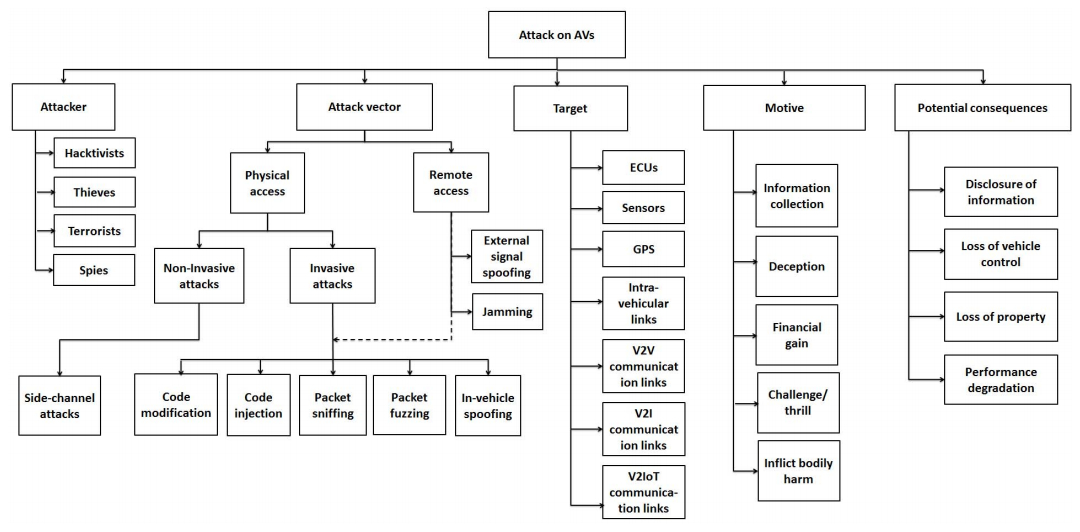
\includegraphics[width=15cm]{img/6.jpg}
	\caption{Autonomous Vehicle Attack Taxonomy \cite{sec}}
	\label{fig:AttackTaxonomy}    
\end{figure}

Another important problem which must to me mentioned while talking about safety and security issues on autonomous cars and is not mentioned in attack taxonomy yet is \textbf{privacy}. An attacker can arrange an attack where he follows car movement, times and makes a very detailed profile about car owner and with this information can do various things: from robbing the house of the victim while he is not at home, to selling this information to someone else, combine different attacks to do the biggest damage attacker want (or is able to) arrange.

\section{Defense against Attacks Taxonomy}

As mentioned earlier it is very hard to predict what is going to happen to prevent yourself against attacks. However, with current knowledge about system and known potential vulnerabilities, it is possible to make some kind of predictions and develop network architectures and working protocols which are not so vulnerable. Various literature surveys propose the main 4 types of defenses for autonomous vehicles: \textbf{Preventive}, \textbf{Passive}, \textbf{Active} and \textbf{Collaborative} defenses. \\
This classification and different ways of protection ensure that the system is secure and resilient for different attacks.

	\begin{enumerate}
		\item \textbf{Preventive Defense}: this type of defense mechanisms mainly focuses on protecting a system from attack before it starts or finishes with success. Preventive defense is mainly focusing on normal working conditions and not during the attack and does not solve any issues with "after attack" scenarios.	
		\begin{enumerate}
			\item \textit{Secure Communication}: for secure communication in any case, from simple chatting to serious control commands, data encryption is basic and crucial. Using encryption content and confidentiality of messages are assured. Encryption scheme can also help with the identification of sender/received of sent data. If the encryption scheme does not include identification, integrity and identification of sender/receiver can be assured, using \gls{MAC} algorithms. To know the integrity and authentication of another side of communication is very important for secure communication.
			\item \textit{In-Vehicle Device Authentication}: controllers used in the car can be completely trusted if they have a manufacturer certificate which gives information such us controller identifier, public key, information about authorized carryout, etc. If information, provided in certificate matches with information which car itself contains, then authentication process is successful and car safely can use all information coming from that particular controller.  
			\item \textit{User Authentication}: sometimes, in order to have more protection, user authentication is used. To make sure that the right person has access to the car (e.g. doors opening, starting the car, etc.) additional biometric information can be used. 
			\item \textit{Firewall}: it is an additional tool, which always can be used. Firewalls check all incoming and outgoing data traffic based on rules which user/authenticated people can define. Firewalls also can be very helpful in communication with a trusted and not-trusted environment: this is very important while communicating with different objects in vehicles' networks.
		\end{enumerate}		
		\item \textbf{Passive Defense}: this type of defense is similar to earlier described preventive defense. Passive defense measures are taken to minimize damage caused by an attacker without having the intention of taking initiative. A passive defense can be an additional level of protection (not the main one). As compared to active defense, the passive defense does not require any analysis from human.		
		\begin{enumerate}
			\item \textit{Attack Detection}:
			\begin{enumerate}
				\item \underline{Intrusion Detection}: To detect physical threats to the car is much easier than to see attacks against system operations. However, there are various models for \gls{IDS} which can be used for autonomous vehicles. Authors of [??, ??] proposed and tested \gls{IDS} models using various computational simulation scenarios. Even though there are models which have quite good results, research and development of \gls{IDS} should not stop in order to achieve higher accuracy in attack detections. 
				\item \underline{Anti-Malware}: these solutions are used in all usual computer network (or only computer) systems. Anti-malware systems need to be able to protect from harmful attempts to penetrate into the main system. Since malware for autonomous cars is a relatively new thing, it might be not possible to find numerous malware "available", but they still should be taken into account. Research communities, who specialize in autonomous cars, trying to predict possible attack models containing new malware to be prepared for these attacks.
			\end{enumerate}
			\item \textit{Attack Response}:
			\begin{enumerate}
				\item \underline{Nullification}: when an attack is recognized by system nullification can be used. This defense mechanism can neutralize an attack using cyber/electronic capabilities, e.g. \gls{GPS} signal anti-jamming technologies [??]. These technologies suppressing signal from malicious jamming devices.
				\item \underline{Isolation}: it helps vehicles to isolate themselves from other cars during an attack. Self-isolation also prevents \glspl{ECU} re-programming while the car is running. Self-isolation should happen in a few levels: the autonomous vehicle network system should isolate itself from other vehicles and the affected layer should be isolated from other levels in the same networking system in order not to affect the healthy vehicle behaviour. When a car is attacked ideally it not only should isolate itself but also inform vehicles around about attack in order other cars could take some actions to defend itself against attack.
			\end{enumerate}
			\item \textit{Attack Recovery}:
			\begin{enumerate}
				\item \underline{Availability}: this feature one of the most important in all types of systems. In the context of autonomous cars, availability is very important when talking about safety inside and outside of the vehicle. In order to ensure safety and have good fault toleration within the system in autonomous cars and to ensure quick recovery after attacks, availability must be ensured in the system.
			\end{enumerate}
		\end{enumerate}				
		\item \textbf{Active Defense}: is one of the advanced and determined defense techniques. Different approached described below.	
		\begin{enumerate}
			\item \textit{Continuous Security Monitoring}: autonomous vehicles belong to critical infrastructure and it is essential that security of these systems should not be compromised. It must have (near) real-time solutions for checking and/or restoring healthy driving conditions in the car. Non-stop and continuous monitoring and "snapshots" of all running systems are required to be available for security checking at any time. It is also important to ensure that all critical devices and interfaces are not blindsided at any time while the car engine is running.			
			\item \textit{Adaptive Security}: Nowadays the most critical systems are fast changing or refer to infrastructure with a fast pace, hence old and static defense mechanisms are not sufficient anymore. It is necessary to model and use defense mechanisms which are dynamic. So-called adaptive reconfigurations for target can be used for ensuring better control and balance during attack. In order to prepare it self for future attacks defense mechanisms should be able to analyze past and current attacks and use self0learning mechanisms to predict what may happen in the future and adapt defense mechanisms for new forms of attack in the future.
		\end{enumerate}				
		\item \textbf{ Collaborative Defense}: 
		\begin{enumerate}
			\item \textit{Cloud Computing}: As mentioned above, if cars in the same network over the \gls{VANET} will share information about potential threats, it is possible that overall security will be improved. When all communication and communication history will be transferred to the clouds, it will become one of the main targets for attackers. Since it will be a "hot spot" for adversaries, security specialist must investigate infrastructure very well, which will give more knowledge and information about potential threats and will let to develop an adaptive defense for better protection of autonomous cars and critical infrastructure.
		\end{enumerate}
	\end{enumerate}

This section provided a brief summary of vulnerabilities, attacks and defense mechanism in term of security of autonomous vehicles. One of the most important things n security is not to stop looking for potential vulnerabilities and ways to protect the car and all network in case of attack and/or to recover as fast as possible if an attack happened. Regardless of the effectiveness of current methods, it is necessary to think about new defense mechanisms for real-time operations of the vehicle. 	

Figure~\ref{fig:DefenseTaxonomy} summaries defense against attacks taxonomy described earlier in this section.

\begin{figure}[h]
	\centering  	
	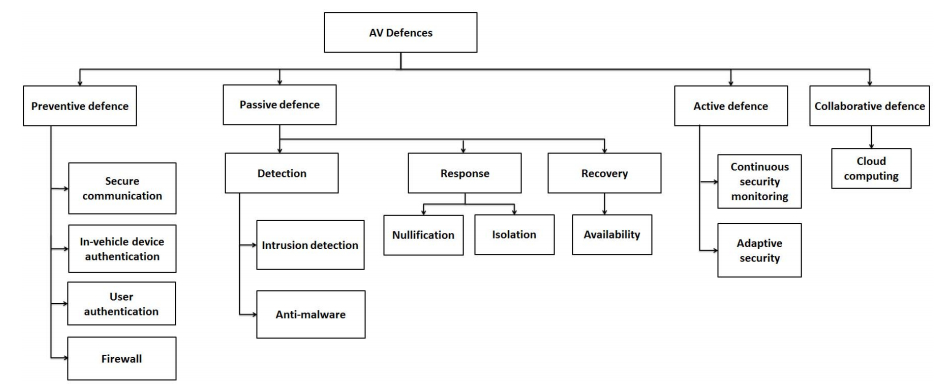
\includegraphics[width=15cm]{img/7.jpg}
	\caption{Autonomous Vehicle Defense Taxonomy \cite{sec}}
	\label{fig:DefenseTaxonomy}    
\end{figure}

\section{The Most Dangerous Attacks}

As mentioned before there are different types of attacks and various ways how to use them. Further in this section will be discussed the most common and dangerous security attacks while making movement prediction: \textbf{visual sensors attacks} and \textbf{privacy issues}.

\subsection{Visual Sensors Attacks}

\subsection{Privacy Issues}

\begin{itemize}
	\item \textbf{Visual sensors attacks}. It is important to make sure that the map of car path is correct and there are no hidden or not real obstacles on the road. \textcolor{red}{(Thinking to write more about External Signal Spoofing on \gls{LiDAR} ???)}
	Another serious attack on visual sensors can be used for a wrong understanding of traffic signs. How easy is to "confuse" STOP sign with Giving Way on Oncoming Traffic sign or to confuse 90km/h with 50km/h, etc.
	\item \textbf{Privacy issue}. Privacy protection might look not important and not relevant while talking about autonomous cars, but it is. \textcolor{red}{(Want to give more insights on how attacks can be arranged and used ??? )}
\end{itemize}

